\scanpage{57}

un pt de $K$ d'ordre $\geq2$, ou d'ordre 1 :

\uline{Lemme} 2 Soi\deleted{\unsure{en}}t $K$ un segment topologique $\subset\mathbb C$, et $x\in K$. \inserted{On suppose $K$ assez régulier (rectifiable suffit ??).} Alors

a) Si $x$ n'est pas extrémité de $K$, alors il existe

\figure{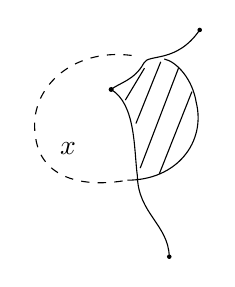
\begin{tikzpicture}[x=0.9cm,y=0.9cm]
\draw[dashed] (0.16,1.02) .. controls (-0.68,1.13) and (-1.30,0.55) .. (-1.20,-0.10) .. controls (-1.15,-0.65) and (-0.63,-0.87) .. (0.10,-0.74);
\draw (0.10,-0.74) .. controls (0.80,-0.74) and (1.21,-0.20) .. (1.07,0.36) .. controls (1.02,0.68) and (0.80,0.93) .. (0.62,0.97);
\draw (1.12,1.38) .. controls (0.79,0.90) and (0.39,1.05) .. (0.33,0.91) .. controls (0.20,0.67) and (-0.02,0.63) .. (-0.13,0.54) .. controls (0.22,0.33) and (0.19,-0.30) .. (0.24,-0.68) .. controls (0.25,-1.21) and (0.68,-1.37) .. (0.69,-1.82);
\draw (0.07,0.39)--(0.34,0.84) (0.22,0.06)--(0.57,0.93) (0.28,-0.57)--(0.82,0.84) (0.55,-0.65)--(1.01,0.51);
\fill (1.12,1.38) circle (.032) (-0.13,.54) circle (.035) (.69,-1.82) circle (.032);
\node at (-.74,-.29) {$x$};
\end{tikzpicture}}

\deleted{un voisinage \inserted{ouvert} $U$ de $x$ dans $\mathbb C$, ne contenant pas d'\unsure{extrémité|extrémités} de $U$, tel que $U\smallsetminus K\cap U$ ait deux composantes connexes $U'$ et $U''$ avec $\overline{U'}\cap U=U'\cup(K\cap U)$, $\overline{U''}\cap U=U''\cup(K\cap U)$, et \unsure{une|qu'une} fonction holo} application continue injective \deleted{de $\unsure{\mathbb D^\circ}$} $H\cap\mathbb D^\circ\longrightarrow\mathbb C$, \deleted{de $H\cap\mathring{\mathbb D}$ dans $\mathbb C$, hol. dans $H\cap\mathring{\mathbb D}$ dans $\mathbb C$, continue} holomorphe dans \deleted{$\mathbb D\smallsetminus\mathbb D\cap\mathbb R$} \inserted{$(\operatorname{Int}H)\cap\mathbb D^\circ$}, \deleted{$=\,]-1,+1[\,=(\unsure{\partial}\mathbb D^{++}\amalg D^{--})$ (mais pas néc\textsuperscript{t} aux deux pts de $\mathbb R$)} (mais pas néc hol. \deleted{dans} aux pts de $\partial H\cap\mathbb D^\circ=\,]-1,+1[$) telle que $f(\partial H\cap\mathbb D^\circ)\subset K$ et $f(0)=x$. De plus, pour une rive donnée de $K$ en $x$, OPS que ladite rive est celle déterminée par \inserted{$\operatorname{Im} f=$} $f(H\cap\mathbb D^\circ)$.

b) Si $x$ est extrémité de $K$, alors $\exists$ $f:H\cap\mathbb D^\circ\longrightarrow\mathbb C$, hol. \inserted{\deleted{et régulière}} dans $(\operatorname{Int}H)\cap\mathbb D^\circ$, \deleted{et injective dans $\unsure{\overline I|I}$ telle que $\unsure{f(-1)=f(1)|f(-t)=f(t)}$ \deleted{\unsure{(sinon)}} soit \unsure{avec} $f:$ telle que $f(0)=0$, $f(]-1,0)$ $f\mid ]-1,0]$ et $f\mid [0,1[$ soient injectifs,}

\figure{\begin{tikzpicture}[x=.8cm,y=.8cm]
\draw[dashed,dash pattern=on 9pt off 4pt] (0.18,1.06) .. controls (-.64,1.14) and (-1.22,.52) .. (-1.18,-.20) .. controls (-1.02,-.96) and (-.45,-1.36) .. (.12,-1.23) .. controls (.94,-1.05) and (1.20,-.28) .. (.98,.54);
\draw (.42,3.13) .. controls (.21,2.41) and (.56,1.78) .. (.28,1.28) .. controls (-.04,.83) and (-.22,.86) .. (.04,.25);
\fill (.04,.25) circle (.027);
\node at (0,-.12) {$x$};
\end{tikzpicture}}
% archive sheet number: 59
